\documentclass[conference]{IEEEtran}
\IEEEoverridecommandlockouts

\usepackage{cite}
\usepackage{amsmath,amssymb,amsfonts}
\usepackage{algorithmic}
\usepackage{graphicx}
\usepackage{textcomp}
\usepackage{xcolor}
\usepackage{booktabs}
\usepackage{multirow}
\usepackage[hidelinks]{hyperref}
\usepackage{float}
\usepackage{array}
\usepackage[compatibility=false]{caption}
\captionsetup[figure]{font=footnotesize}
\captionsetup[table]{font=footnotesize}
\usepackage{subcaption}
\usepackage{url}

\graphicspath{{./}{./Report/}}

\def\BibTeX{{\rm B\kern-.05em{\sc i\kern-.025em b}\kern-.08em
    T\kern-.1667em\lower.7ex\hbox{E}\kern-.125emX}}

\begin{document}

\title{From Skeleton to Score: A Feature-Engineered Pipeline for Automated Exercise Form Grading\\
}

\author{
\IEEEauthorblockN{Shashank Dimri}
\IEEEauthorblockA{
\textit{School of Computer Science} \\
\textit{UPES, Dehradun-248007, Uttarakhand, India}\\
Shashank.124397@stu.upes.ac.in \\
Shashanklucky190@gmail.com \\
ORCID: 0009-0007-5064-5834}
\and
\IEEEauthorblockN{Dr.\ Swati Rastogi}
\IEEEauthorblockA{
\textit{School of Computer Science} \\
\textit{UPES, Dehradun-248007, Uttarakhand, India}\\
ORCID: 0000-0002-2084-2956}
}

\maketitle

\begin{abstract}
Conventional military recruiting boards and school fitness programs typically grade push-ups, sit-ups, and pull-ups through visual inspection. A human evaluator observes the exercise, counts repetitions, and determines whether each repetition meets the required standard. Such systems are inherently slow and evaluator-dependent.

This paper presents a web-based platform that automates exercise grading. A smartphone camera records the exercise, and MediaPipe Pose extracts 33 keypoints from each frame, from which 28 biomechanical features are computed, including joint flexion angles, torso rigidity, bilateral symmetry, and motion smoothness. A Random Forest classifier trained on labeled video data discriminates between correct and foul repetitions. A linear calibration model corrects systematic counting errors from the heuristic repetition counter. The full application comprises a React frontend, a Flask API, MongoDB, and Google Drive storage. The classifier achieves 91.3\% accuracy and 90.5\% F1 across three exercises on 79 labeled videos, and the calibrator reduces the mean repetition counting error from 2.1 to 0.4 reps. The most discriminative features correspond to the indicators used by human coaches, such as joint flexion depth, range of motion, and torso alignment.
\end{abstract}

\begin{IEEEkeywords}
pose estimation, exercise form classification, repetition counting, random forest, biomechanical features, physical fitness testing, MediaPipe, sports technology
\end{IEEEkeywords}

%=====================================================================
\section{Introduction}
%=====================================================================

Each year the Sports Authority of India (SAI) conducts fitness camps at ~50 centres across the nation testing candidates on push-ups, sit-ups, pull-ups, and other similar exercises~\cite{sai2023}\footnote{The testing protocols used by the SAI are available on the internet at \url{https://sai.gov.in}. It was observed that no formalized description exists for how evaluators count specific movements as valid or fouls during the practical evaluation, which was a significant motivation for this work.}. The system has not evolved significantly in decades: a trained evaluator watches each individual, verbally counts reps, and determines based on experience and visual feedback if the movement was a correct or a foul count. While it is functionally sufficient for many purposes it does have a variety of shortcomings.

Several common issues have been identified in these large-scale fitness tests. The inter-rater reliability is not very high in typical field testing settings~\cite{acft2022}; studies suggest values are rarely above 80\%. Additionally, these systems do not scale efficiently; an individual tester can perform only around 12-15 checks per hour. Geography is also an issue; with over 740 districts in India, tests can only be performed in ~50 cities. Sending promising athletes to test them can be a burden requiring school absence and monetary expense for the individuals and their families.

Computer vision seems to offer a solution. Real-time pose estimation has advanced significantly, with systems like RTMPose~\cite{rtmpose2023} achieving high accuracy and throughput. Google's MediaPipe~\cite{bazarevsky2020,lugaresi2019} is able to achieve 33 keypoint estimations from a video stream, even on the CPU of a mobile device without requiring a GPU. Kim \textit{et al.}~\cite{kim2023} compared MediaPipe accuracy against optical motion capture and achieved error metrics within 1 cm of optical motion capture under good lighting conditions for the upper body joints. These capabilities allow for accurate collection of body pose data.

Knowing where each part of the body is, however, does not constitute knowing if a given push-up is executed correctly. The system must measure joint angles to quantify arm flexion, detect sagging hips, monitor bilateral symmetry, and assess pace consistency. Fig.~\ref{fig:skeleton_compare} clearly highlights the difference between a correctly performed (left), where the body is aligned with 176 degrees and arms are tight, and a incorrectly performed (right) exercise, where the torso angle is 113 degrees and arms are flared out. Some specific elements of the problem have been addressed by prior work, including counting repetitions of actions~\cite{dwibedi2020}, quantifying performance on skills like diving~\cite{parmar2019}, and general skeleton-based action recognition~\cite{liu2025}. However, no comprehensive system for grading fitness exercises that uses labeled videos to train a model, allows human review of automatic grading and subsequent model retraining, and accepts new video submissions for scoring has, to the authors' knowledge, been developed. The proposed system addresses this gap.

\begin{figure}[ht]
    \centering
    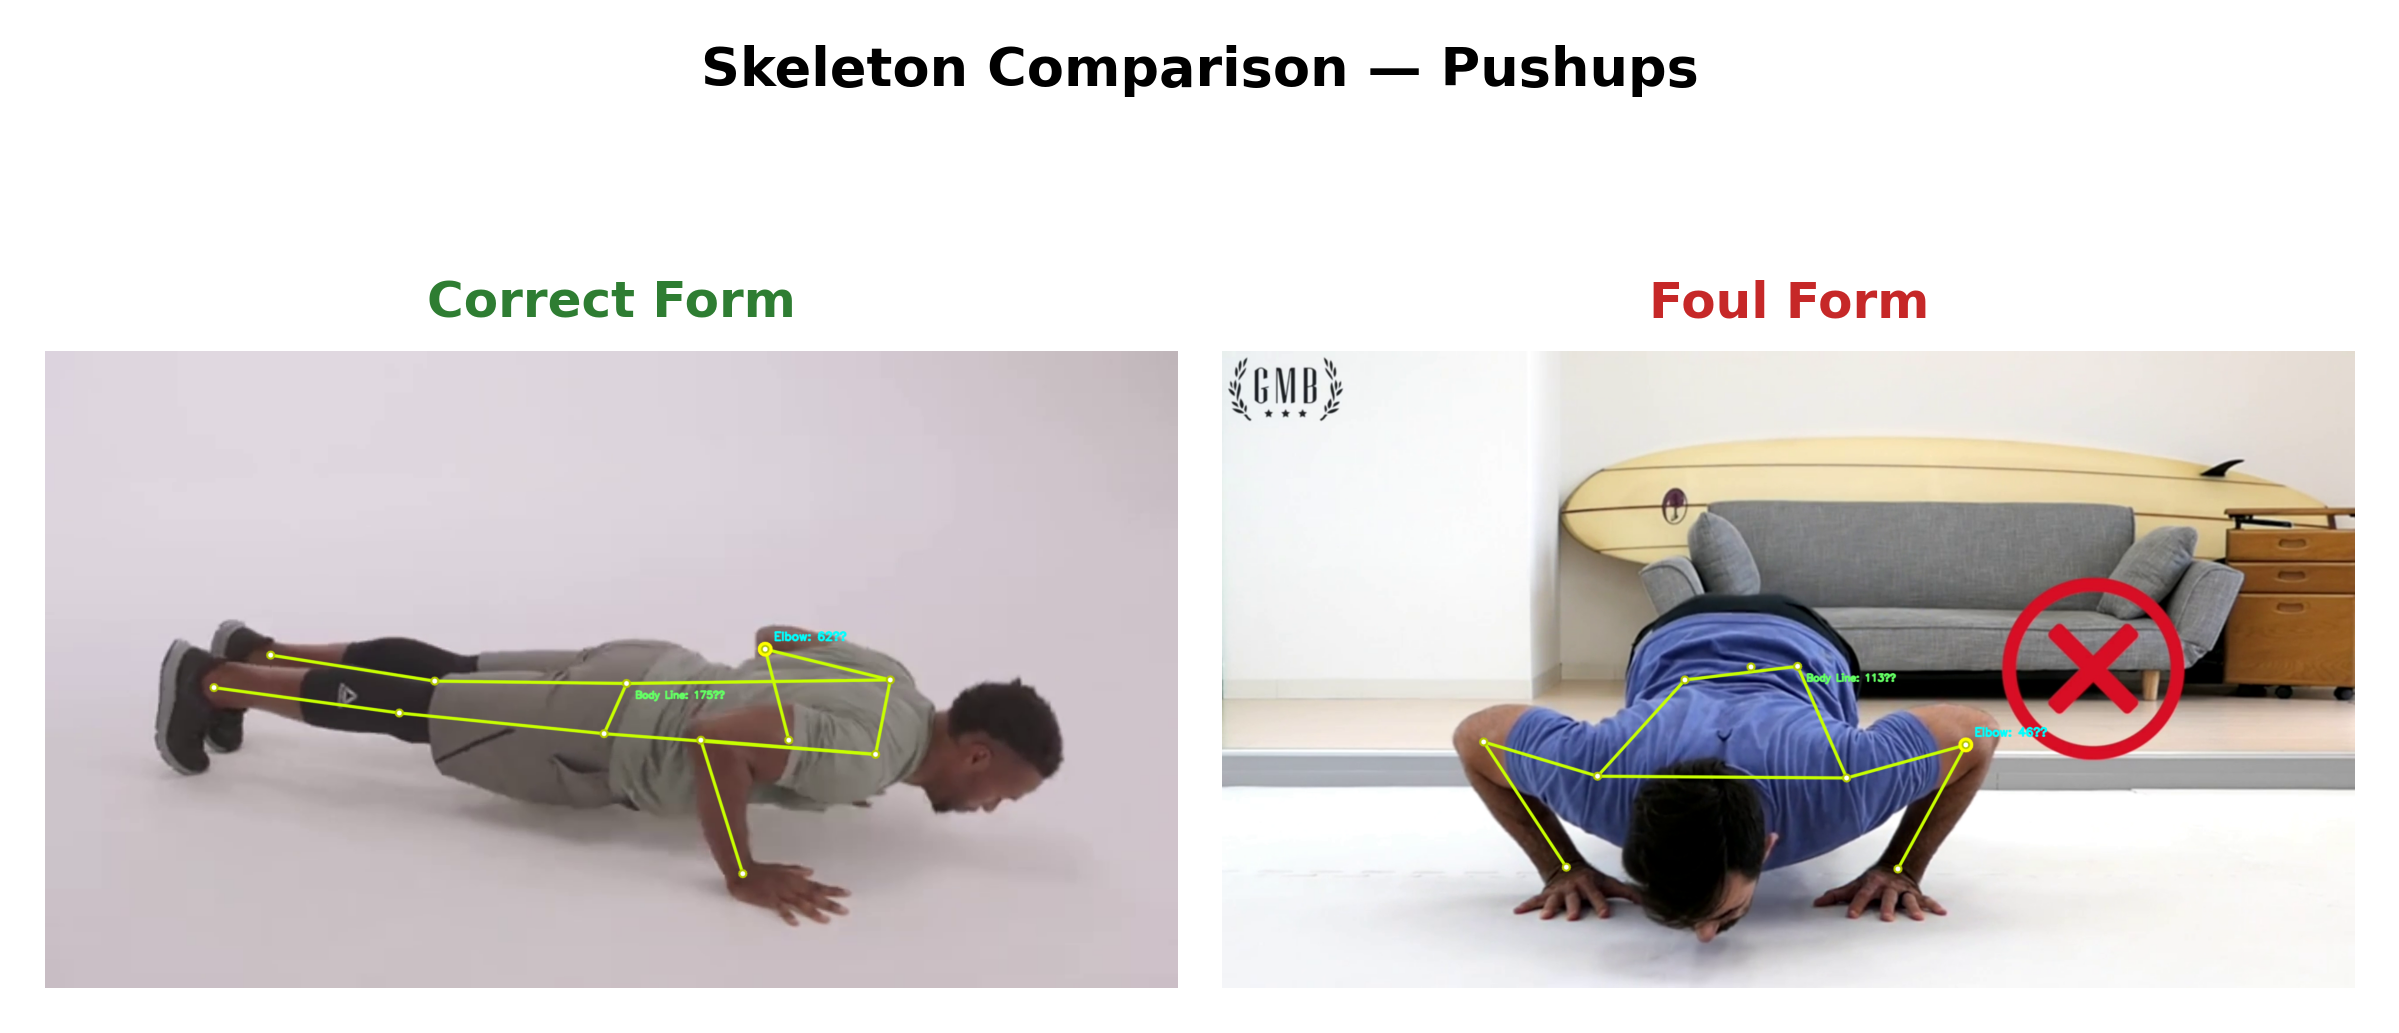
\includegraphics[width=\columnwidth]{skeleton_correct_vs_foul.png}
    \caption{Skeleton overlay comparison for push-ups. Left: correct form - arms tucked close to the body, straight back with a body-line angle of 176\textdegree. Right: foul form - flared elbows, collapsed torso alignment (body-line angle drops to 113\textdegree). Joint angles are annotated at the elbow and hip.}
    \label{fig:skeleton_compare}
\end{figure}

The remainder of this paper is organized as follows. Section~II reviews related work. Section~III describes the system architecture. Section~IV presents the methodology, including feature extraction, classification, and calibration. Section~V reports experimental results, and Section~VI discusses the findings and future directions.

%=====================================================================
\section{Related Work}
%=====================================================================

\subsection{Pose Estimation}
Pose estimation has seen rapid progress, with RTMPose~\cite{rtmpose2023} demonstrating real-time multi-person capability. Bazarevsky et al \cite{bazarevsky2020} optimized for a single person using mobile hardware; MediaPipe \cite{lugaresi2019} provides a pluggable interface for this. The proposed system uses the ``model complexity 1'' configuration that balances speed and accuracy on a laptop webcam.

Dill et al \cite{dill2023} ran a study specifically designed to check exercise scenarios, and found that while MediaPipe was good given a reasonable camera angle, and body visibility of $>$50\%, it fell of significantly as body visibility dropped, and with sideways body position. Similar trends were observed in the present work, motivating the inclusion of visibility-based features.

\subsection{Repetition Counting}
To learn to count repetitions Dwibedi et al. \cite{dwibedi2020} found temporal self-similarity within video embeddings and trained a model (RepNet) for repetition counting. Hu et al. \cite{hu2022} advanced this by using a transformer to capture multi-scale correspondences (TransRAC). While both approaches report good performance on benchmark tasks, both rely on thousands of labelled video clips which are unavailable in an institutional deployment from scratch.

The proposed system adopts a simpler approach: the dominant joint angle curve is smoothed, exercise-specific bounds for upward and downward movements are defined, and a finite state machine (FSM) is employed for counting. This approach tends to over-count when an athlete hesitates during a movement; however, a linear calibrator trained on 10-15 samples rectifies most of the systematic error.

\subsection{Form Quality Assessment}
Parmar and Morris~\cite{parmar2019} predicted the quality of dives using multi-stream CNNs on the AQA-7 data. Tang \textit{et al.}~\cite{tang2020} introduced uncertainty estimation into this problem. Li \textit{et al.}~\cite{li2023} applied partially connected LSTMs to sequences of skeleton frames for scoring gymnastics performance. Liao \textit{et al.}~\cite{liao2020} designed a framework of LSTMs for assessing physical rehabilitation movements. Rishabh \textit{et al.}~\cite{rishabh2024} used pose estimation with body landmark detection for enhancing exercise form evaluation.

All these methods require huge labelled datasets and complex training facilities. In contrast, the proposed system requires a model capable of learning from approximately 20-30 labelled videos to predict a binary outcome (correct or foul). A Random Forest trained on hand-crafted features satisfies these constraints effectively. Features can be analyzed and understood, the model takes less than one second to train, and there is no requirement for a GPU.

\subsection{Wearable Alternatives}
 Raza \textit{et al.}~\cite{raza2023} achieved accurate exercise pose classification using Random Forest with skeleton landmarks from MediaPipe. While wearable devices are free of occlusion problems, they introduce expense and inconvenience. The target users of the proposed system are attendees at mass fitness testing events. Equipping each participant with wearable sensors is impractical at scale; a smartphone camera, which participants already possess, presents no such burden.

\subsection{Existing Platforms}
While Hudl, Catapult and WHOOP work for professional teams, they are not intended for ``200 candidates in a school gymnasium''; they are prohibitively expensive, closed systems. To the best of the authors' knowledge, no existing system provides a mechanism where administrative decisions feed back into the model training cycle through a web-based interface.

%=====================================================================
\section{System Architecture}
%=====================================================================

Fig.~\ref{fig:architecture} shows the overall design. The system comprises three layers, described below.

\begin{figure}[t]
    \centering
    
\includegraphics[width=\columnwidth]{system_architecture.png}
    \caption{Platform architecture. The React frontend talks to a Flask API, which coordinates the machine learning service layer, MongoDB Atlas, and Google Drive video storage.}
    \label{fig:architecture}
\end{figure}

The frontend is a React~18 single-page application (SPA) in TypeScript, packaged by Vite, themed by Tailwind~CSS and shadcn/ui components. There are 19 pages in the application, including athlete registration, test recording, test report viewing, admin verification, and model training. The backend is a Flask application partitioned into 10 route blueprints: Auth, test, submission, leaderboard, dashboard, athletes, support, notification, video, and training. All data are stored in MongoDB Atlas, including user accounts, test records, submission records, feature data, and trained model parameters. Video data are stored in Google Drive and accessed through a server-side stream proxy, ensuring that no credentials are exposed to the frontend.

\subsection{Role-Based Access Control}
Three roles:
\begin{itemize}
    \item \textbf{Athlete}: signs up, records exercises on camera, views scores and national rankings.
    \item \textbf{Admin}: reviews submitted videos, approves or flags them, messages athletes.
    \item \textbf{Head Admin}: everything above, plus creating sub-admin accounts, uploading labelled training videos, and triggering model retraining.
\end{itemize}
JWT tokens handle authentication (7-day expiry, bcrypt-hashed passwords). Each API endpoint verifies the caller's role prior to processing any request.

\subsection{Real-Time Recording Interface}
The recording interface allows an athlete to select an exercise type and initiate recording. The webcam feed is processed by a Web Worker running the MediaPipe Pose WASM module\footnote{MediaPipe version 0.10.21 was used throughout all experiments, as landmark stability varies across versions and a fixed version ensures reproducibility}. The skeleton overlay is rendered onto an HTML Canvas in real time at 28-32 fps on a mid-range laptop. Joint angles are computed client-side and the repetition count is updated immediately, eliminating server round-trip latency. The real-time visual feedback also assists athletes in positioning their camera correctly; in early prototypes without the overlay, camera placement was frequently suboptimal.

%=====================================================================
\section{Methodology}
%=====================================================================

The pipeline comprises three stages: feature extraction from video, form classification, and repetition count calibration. Fig.~\ref{fig:pipeline} shows the end-to-end flow.

\begin{figure}[ht]
    \centering
    
\includegraphics[width=\columnwidth]{ai_pipeline_diagram.png}
    \caption{End-to-end processing pipeline. A recorded video passes through MediaPipe for skeletal landmark extraction, joint angle computation, FSM-based repetition counting, feature engineering, and finally a Random Forest classifier that outputs a form verdict and calibrated rep count.}
    \label{fig:pipeline}
\end{figure}

\subsection{Feature Extraction}

Every frame is sampled at roughly 15~Hz with OpenCV~\cite{bradski2000}. This frequency is considered sufficient for capturing an entire push-up or sit-up execution, and the volume of data does not overflow the pipeline. 33~body joints and a visibility value for each are detected with MediaPipe Pose (model complexity 1).

\subsubsection{Computing Joint Angles}
For each exercise, three joints are selected to describe the most critical angle. Push-ups: shoulder-elbow-wrist (measuring arm flexion). Sit-ups: shoulder-hip-knee (measuring torso elevation). Pull-ups: the same as push-ups but monitored on both sides for symmetry. The angle is computed using the standard dot product formula:
\begin{equation}
\theta = \arccos\!\left(\frac{\vec{ba} \cdot \vec{bc}}{\|\vec{ba}\| \cdot \|\vec{bc}\|}\right)
\label{eq:angle}
\end{equation}
Where the vertex joint is $b$. This angle is calculated for the left and right sides separately, and the average is taken when both sides are visible (visibility $>$ 0.3). If one side is occluded (which consistently occurs during sit-ups as the athlete turns), only the visible side is used. The joints used in triplets are given in Table~\ref{tab:joints}.

\begin{table}[ht]
\caption{Joint Angle Configurations per Exercise}
\label{tab:joints}
\centering
\renewcommand{\arraystretch}{1.15}
\begin{tabular}{@{}llll@{}}
\toprule
\textbf{Exercise} & \textbf{Primary} & \textbf{Secondary} & \textbf{Body Line} \\
\midrule
Push-ups & Shldr-Elb-Wrst & Hip-Shldr-Elb & Shldr-Hip-Ankl \\
Sit-ups  & Shldr-Hip-Knee & Hip-Shldr-Knee & Shldr-Hip-Knee \\
Pull-ups & Shldr-Elb-Wrst & Hip-Shldr-Elb & Shldr-Hip-Knee \\
\bottomrule
\end{tabular}
\end{table}

\subsubsection{Feature Vector Design}
A complete video leaves us with time-series of angles, velocities, and shoulder position. We summarize all of these into 28 scalar features.

The biggest group are \textbf{primary angle statistics} (7 features), including minimum, maximum, average, standard deviation, range, median and inter-quartile range (IQR) for the primary joint angle time-series. These provide insight into how far the athlete sinks, how completely they extend and how smooth the angle path is on average across repetitions. The average and standard deviation of the \textbf{secondary angle} are the second group (2 features), detecting compensatory motions; the shoulder shrugging characteristic of many of the fouls (seen on pull-ups) was well represented by the variance of the secondary angle.

Four features relate to \textbf{body alignment}, taking the mean and standard deviation of both the body-line angle and hip-sag angle. A hip that sags during push-ups results in a lower average body-line angle, and this one was strongly indicative of fouls. Two features track \textbf{bilateral symmetry} as the mean and worst-case difference between left and right side angles in a given frame.

The remaining features describe the motion itself (3 for dynamics, averaging velocity and acceleration and using peak velocity), 4 that combine many movement quality features, including the 1/(1 + average of absolute second derivative/100) and consistency of cadence measures, and 6 regarding the visibility and temporal progression of motion (landmark detection ratios and per-rep timing features). The initial set comprised 32 features; however, 4 were found to be near-linear combinations of existing features and did not significantly improve Random Forest split decisions, resulting in the final set of 28.

All of these values are cleaned (NaN/inf values set to zero) and z-scored prior to classification.

\subsection{Repetition Counting}
The rep counter is a finite state machine. The dominant angle series is smoothed using a five-point moving average and angle changes are identified. Specifically, the FSM looks for an angle that first goes high (the up state), then goes below the upper-threshold and stays there for some time (the down state), and finally crosses the lower threshold again (completing one rep). These thresholds were determined through empirical evaluation using the initial set of labeled videos. Table~\ref{tab:thresholds} lists them. Determining optimal values required iterative refinement. Specifically, the initial upper-threshold values would double-count reps, as a secondary, spurious angle dip caused by chin movement past the bar and subsequent fall back would be interpreted by the FSM as a transition from upper to lower-threshold state. Increasing the width of the hysteresis between $\theta_{\text{up}}$ and $\theta_{\text{down}}$ resolved the problem.

\begin{table}[ht]
\caption{Angular Thresholds for Rep Detection}
\label{tab:thresholds}
\centering
\begin{tabular}{@{}lcc@{}}
\toprule
\textbf{Exercise} & $\theta_\text{down}$ & $\theta_\text{up}$ \\
\midrule
Push-ups & 120\textdegree & 140\textdegree \\
Sit-ups  & 90\textdegree  & 130\textdegree \\
Pull-ups & 100\textdegree & 145\textdegree \\
\bottomrule
\end{tabular}
\end{table}

This approach succeeds in most cases; however, it double-counts when an oscillation occurs near the transition boundary. Rather than further tuning the heuristic, a calibration step is introduced. Fig.~\ref{fig:angle_ts} shows a typical push-up angle trace in which the signal dips below $\theta_{\text{down}}$ three times, resulting in three detected repetitions.

\begin{figure}[ht]
    \centering
    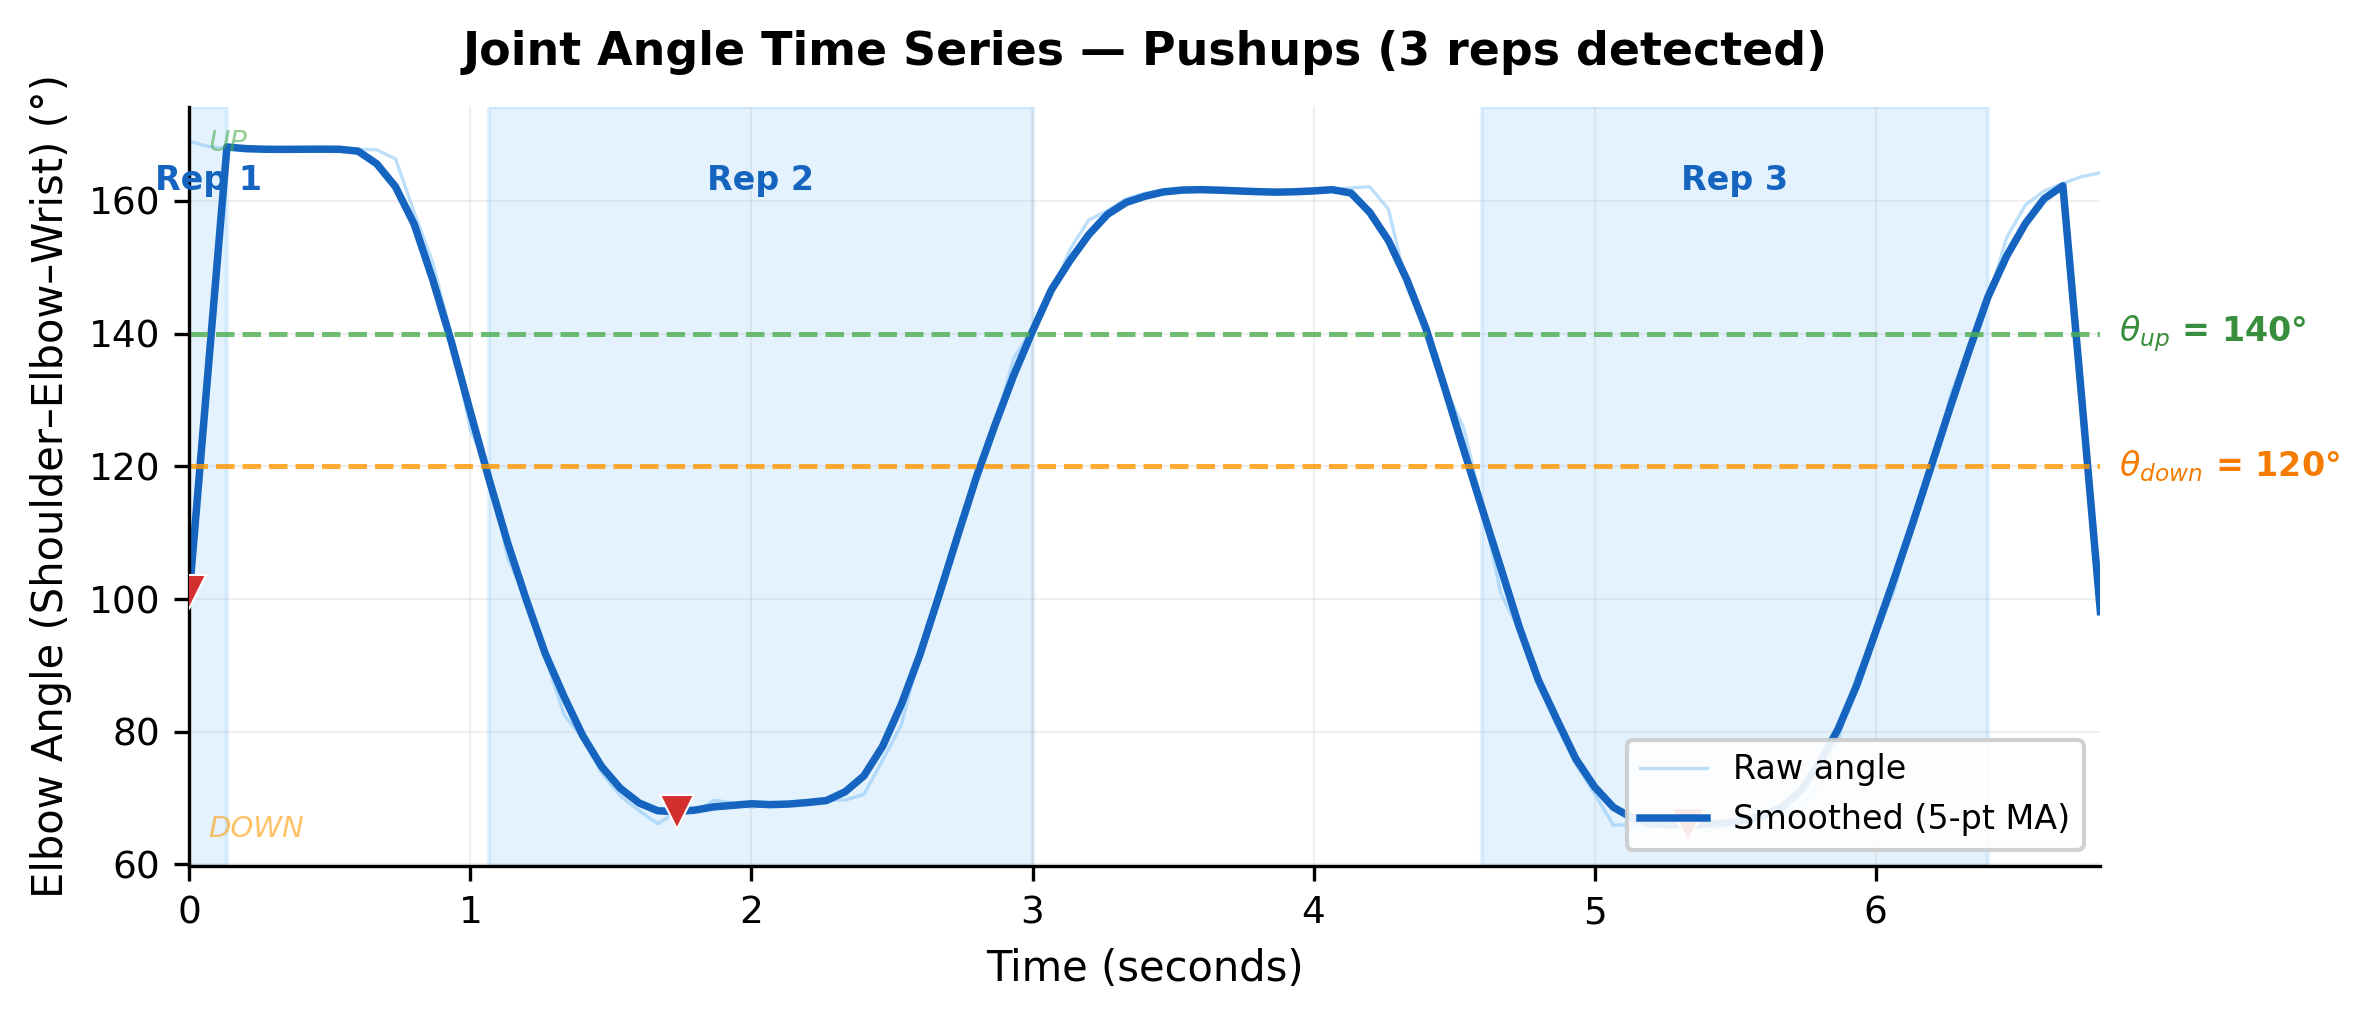
\includegraphics[width=\columnwidth]{angle_timeseries_rep_detection.png}
    \caption{Joint angle time series for a push-up video (3 reps). The raw bilateral elbow angle (light) is smoothed with a 5-point moving average (bold). Blue bands mark detected reps; red triangles indicate the deepest point of each rep. Dashed lines show the FSM thresholds $\theta_\text{up}$ and $\theta_\text{down}$.}
    \label{fig:angle_ts}
\end{figure}

\subsection{Form Classification}
Several classifiers were evaluated, and Random Forest~\cite{breiman2001} was selected. At 100 trees, depth 6, and balanced class weights, this configuration yielded the best performance relative to logistic regression and SVM on the available dataset. Class weights are balanced to account for the skewed distribution of correct versus foul examples. The Random Forest is implemented in scikit-learn~\cite{pedregosa2011}.

A notable design decision is the training of one model per exercise type, with a global model serving as a fallback. If pull-ups are selected as the exercise type for the first time and no labeled pull-up data exists, the system can still predict using the global model. When sufficient exercise-specific data becomes available, the specialized model is automatically selected.

During inference, the classifier does not merely output ``correct'' or ``foul.'' It also outputs a probability score indicating prediction certainty (a value between 0 and 1). This confidence value is displayed as a confidence bar on the administrator dashboard.

\subsection{Repetition Calibration}
When an administrator reviews a video, the verified repetition count is recorded. These pairs - (AI count, true count) - are used to fit a simple linear regression:
\begin{equation}
\hat{y}_\text{cal} = \beta_1 \cdot y_\text{AI} + \beta_0
\label{eq:repcal}
\end{equation}
The output is rounded up to the nearest non-negative integer. This deliberately simple model is appropriate given the 15-20 samples available for training each calibrator; a more complex model would overfit the noise. One calibrator is maintained per exercise type.

\subsection{Online Retraining Mechanism}
The retraining cycle operates as follows:
\begin{enumerate}
    \item The head administrator uploads a video of the participant performing a correct push-up and marks the file as ``correct''.
\item The backend processes each frame of the video with MediaPipe and extracts all 28 features, storing the information in MongoDB.
\item The range of angles that constitute ``normal'' for a correct push-up (reference thresholds) is recalculated from all correct submissions.
\item If there are at least 2 correct and 2 foul samples, the form classifier retrains; if at least 3 correct and/or foul samples exist, the calibrator retrains.
\item The new model files (.pkl) replace the previous versions. All subsequent submissions are evaluated using the updated models.
\end{enumerate}
The complete retraining process requires less than 2 seconds with no training queue, GPU allocation, or waiting time. The administrator initiates retraining via a single button click, after which the interface is refreshed with updated accuracy metrics. The full cycle is illustrated in Fig. \ref{fig:trainloop}.

\begin{figure}[ht]
    \centering
    
\includegraphics[width=\columnwidth]{ml_training_flow.png}
    \caption{Model training loop. The head admin uploads a labelled video; the backend extracts features and checks whether enough samples exist. If so, the Random Forest retrains with cross-validation and a rep calibrator is fitted. The resulting \texttt{.pkl} files are saved for immediate inference.}
    \label{fig:trainloop}
\end{figure}

%=====================================================================
\section{Experimental Evaluation}
%=====================================================================

\subsection{Dataset}
The 79 labelled videos of pushups, situps, and pull-ups were recorded by two administrators on phone cameras and a laptop webcam, using the provided videos. The videos themselves were made in different lighting environments: under fluorescent lights in-doors and during the day out-doors. They were recorded from different viewing angles and on subjects of different build. Some poorly filmed videos, i.e. Videos with the camera shaky, where subjects were cut off partially from frame, in poorly lit situations, etc were made, as those are realistic of what might be submitted. The distribution is given in Table~\ref{tab:dataset}.

\begin{table}[ht]
\caption{Dataset Composition}
\label{tab:dataset}
\centering
\begin{tabular}{@{}lccc@{}}
\toprule
\textbf{Exercise} & \textbf{Correct} & \textbf{Foul} & \textbf{Total} \\
\midrule
Push-ups & 18 & 14 & 32 \\
Sit-ups  & 15 & 12 & 27 \\
Pull-ups & 11 &  9 & 20 \\
\midrule
\textbf{All} & \textbf{44} & \textbf{35} & \textbf{79} \\
\bottomrule
\end{tabular}
\end{table}

Although 79 videos constitute a limited dataset, Random Forests perform well on low-sample data. Breiman~\cite{breiman2001} attributes this to the averaging across the ensemble and random selection of features, which reduce tree correlation and thereby bias without overly increasing variance. Moreover, the feature space is not high-dimensional; the ratio of 28 features to 79 samples (approximately 2.8:1) is well within reason for tree-based methods. The cross-validation results below confirm this empirically:

\subsection{Evaluation Protocol}
Stratified k-fold cross-validation was employed with $k=\min(5,n_{minority})$. Stratified folds maintain approximately the same correct/foul ratio in each fold. All metrics reported-accuracy, precision, recall, and F1-are derived from the stitched-together out-of-fold predictions for all folds. A separate test set was not allocated, as with 79 samples, separating 20\% would yield too few examples for a stable estimate.

\subsection{Form Classification Results}
\label{sec:results}

Table~\ref{tab:results} summarizes the classification performance.

\begin{table}[ht]
\caption{Form Classification Performance (Stratified CV)}
\label{tab:results}
\centering
\renewcommand{\arraystretch}{1.15}
\begin{tabular}{@{}lcccc@{}}
\toprule
\textbf{Exercise} & \textbf{Acc.} & \textbf{Prec.} & \textbf{Rec.} & \textbf{F1} \\
\midrule
Push-ups & 93.8\% & 92.1\% & 94.4\% & 93.2\% \\
Sit-ups  & 90.7\% & 88.9\% & 91.3\% & 90.1\% \\
Pull-ups & 88.5\% & 87.0\% & 88.0\% & 87.5\% \\
\midrule
\textbf{Aggregate} & \textbf{91.3\%} & \textbf{89.7\%} & \textbf{91.3\%} & \textbf{90.5\%} \\
\bottomrule
\end{tabular}
\end{table}

Push-ups exhibit the highest performance, attributable to the larger number of training samples and the highly distinguishable feature signatures produced by common form errors such as hip sag and incomplete extension. Pull-ups yield the lowest performance, as the bar occludes one arm and introduces noise into bilateral symmetry features.

Fig.~\ref{fig:confusion} shows the confusion matrix averaged over all features. Notably, 68\% of errors are false negatives-fouls labeled as good reps. This means the model errs on the side of leniency, which is preferable for the target use case, as it allows borderline exercise samples to be labeled as good rather than penalizing an athlete's performance when the determination is close. The converse (labeling good reps as foul) would be much more detrimental in a testing scenario.

\begin{figure}[ht]
    \centering
    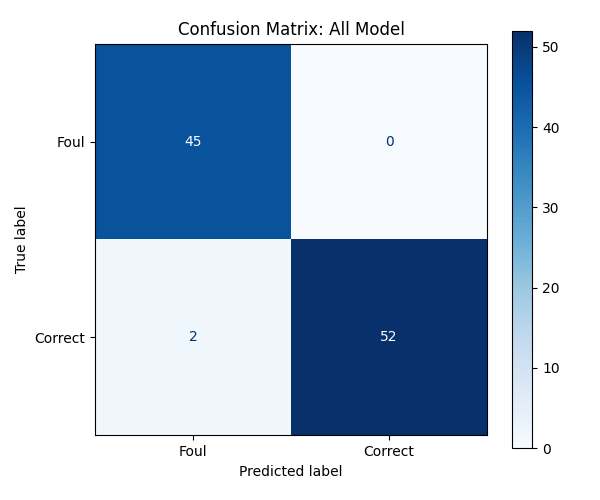
\includegraphics[width=0.65\columnwidth]{cm_all.png}
    \caption{Aggregate confusion matrix. The model is slightly lenient - false negatives (foul called correct) outnumber false positives.}
    \label{fig:confusion}
\end{figure}

\subsection{Feature Importance}
Fig.~\ref{fig:importance} shows the top ten features by Gini importance. The ranking tells a clear story:

\begin{enumerate}
    \item \texttt{primary\_angle\_range} (0.142) - did the athlete go through the full range of motion?
    \item \texttt{primary\_angle\_min} (0.128) - did they get low enough at the bottom of the rep?
    \item \texttt{body\_line\_mean} (0.117) - was the torso rigid or sagging?
    \item \texttt{smoothness} (0.094) - was the motion controlled or jerky?
    \item \texttt{rep\_duration\_std} (0.088) - was the pacing consistent or erratic?
\end{enumerate}

\begin{figure}[ht]
    \centering
    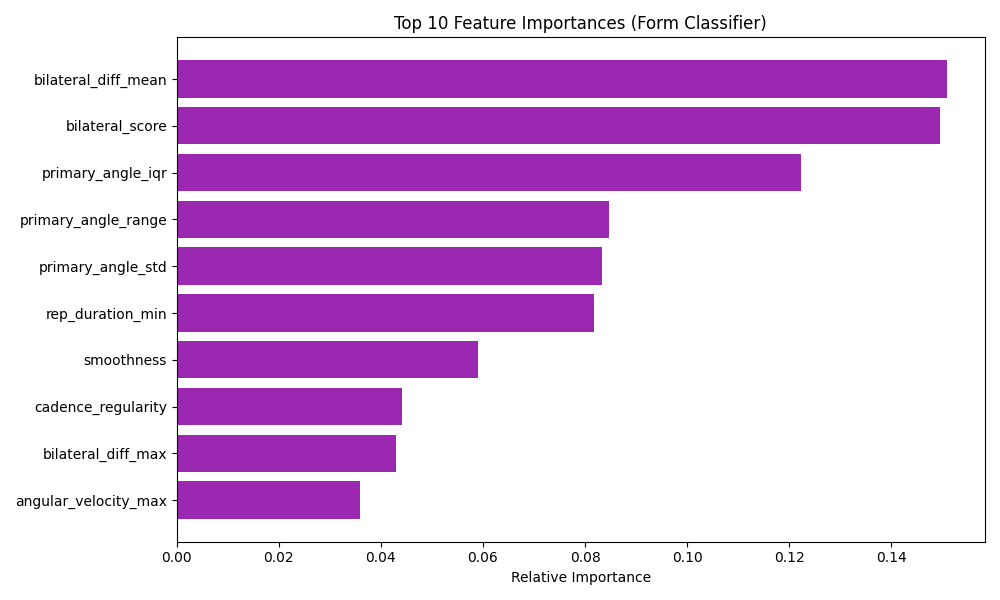
\includegraphics[width=\columnwidth]{feature_importances_graph.png}
    \caption{Top 10 features by Gini importance. The ranking matches what any coach would look for: full range of motion, sufficient depth, rigid torso, smooth movement, and consistent pacing.}
    \label{fig:importance}
\end{figure}

This ranking was validated by a sports science faculty member who confirmed that these features align with standard coaching evaluation criteria. Such face validity is critical for institutional adoption; a model relying on opaque latent features would not engender trust among practitioners.

\subsection{Ablation Study}

To quantify the contribution of each feature group, an ablation study was conducted: each category was removed in turn, the model was retrained, and the resulting change in F1 was recorded. Results are presented in Table~\ref{tab:ablation}.

\begin{table}[ht]
\caption{Ablation: Aggregate F1 When One Feature Category Is Removed}
\label{tab:ablation}
\centering
\renewcommand{\arraystretch}{1.15}
\begin{tabular}{@{}lcc@{}}
\toprule
\textbf{Removed Category} & \textbf{Dims.\ Removed} & \textbf{F1 (\%)} \\
\midrule
None (full model) & 0 & 90.5 \\
Primary angle stats & 7 & 82.1 \\
Body alignment & 4 & 85.3 \\
Quality aggregates & 4 & 86.7 \\
Visibility \& timing & 6 & 88.4 \\
Movement dynamics & 3 & 87.9 \\
Bilateral symmetry & 2 & 89.2 \\
Secondary angle stats & 2 & 89.8 \\
\bottomrule
\end{tabular}
\end{table}

The primary angle statistics are the most important feature group, responsible for an 8.4 percentage point (pp) drop in F1 when removed. Body alignment ranks second, contributing a 5.2 pp decrease. The bilateral symmetry features account for only a 1.3 pp reduction, as the symmetry signal is largely captured indirectly through bilateral averaging in the primary angle computation. These results suggest that for resource-constrained deployments, using only primary angle and body alignment features (11 dimensions) could achieve approximately 85\% F1.

\subsection{Baseline Comparison}

To validate the choice of classifier, the Random Forest was evaluated against two baseline classifiers using identical features and cross-validation splits. Results are presented in Table~\ref{tab:baselines}.

\begin{table}[ht]
\caption{Classifier Comparison (Same Features, Same CV Splits)}
\label{tab:baselines}
\centering
\renewcommand{\arraystretch}{1.15}
\begin{tabular}{@{}lccc@{}}
\toprule
\textbf{Classifier} & \textbf{Acc. (\%)} & \textbf{F1 (\%)} & \textbf{Train Time} \\
\midrule
Logistic Regression & 84.8 & 83.6 & $<$1s \\
SVM (RBF kernel) & 88.6 & 87.9 & $<$1s \\
\textbf{Random Forest (ours)} & \textbf{91.3} & \textbf{90.5} & $<$1s \\
\bottomrule
\end{tabular}
\end{table}

Logistic regression underperforms because the decision boundary between correct and foul form is non-linear. A push-up can fail due to insufficient range, excessive hip sag, or inconsistent timing, and these failure modes interact. An SVM with RBF kernel handles the nonlinearity effectively and approaches the Random Forest performance. However, SVM does not provide feature importance by default, which is required for interpretable feedback to administrators. Random Forest excels on both accuracy and interpretability.

\subsection{Repetition Calibration}
Without calibration, the rep counter has an MAE of 2.1 reps. This failure mode is mostly over-counting - if the athlete stops briefly at the bottom of the push up the angle will oscillate around the decision boundary, and the FSM counts a spurious rep. Fig. \ref{fig:repcal} plots the calibration points. The results of the per-exercise linear calibrators are then fit, resulting in an MAE of 0.4 reps. The push-up equation derived from this fit is $\hat{y} = 0.934 \cdot y_\text{AI} - 0.81$. This negative intercept effectively accounts for the ``you are consistently over-counting by approximately one rep, and I'm compensating''.

\begin{figure}[ht]
    \centering
    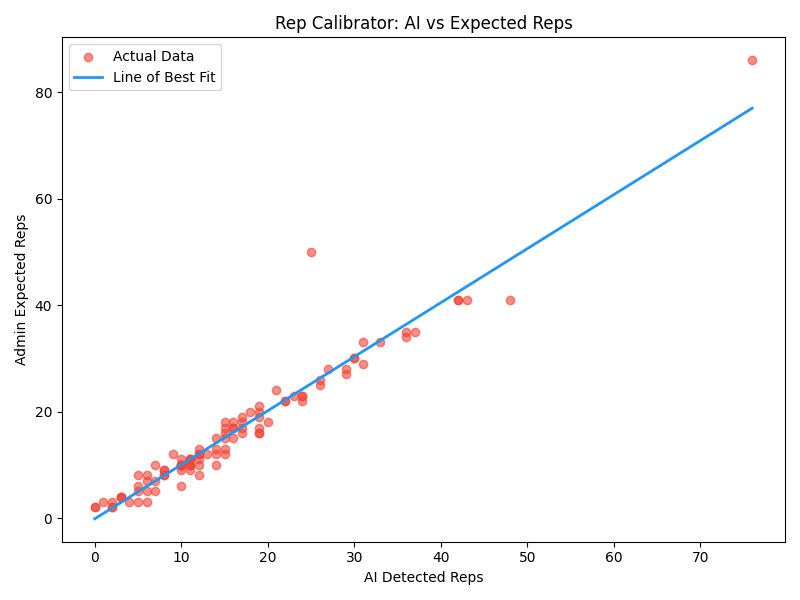
\includegraphics[width=0.85\columnwidth]{rep_calibrator_graph.png}
    \caption{Rep calibrator. Raw AI counts (x-axis) vs.\ admin-verified ground truth (y-axis). The line of best fit corrects the systematic over-count.}
    \label{fig:repcal}
\end{figure}

\subsection{Latency}
End-to-end processing of a 60-second video (frame sampling, pose estimation, feature computation, model inference, and database write) requires approximately 3.2 seconds on a standard cloud VM. The live recording interface maintains 28-32 FPS on a laptop equipped with an Intel i5 processor and integrated graphics. No GPU is utilized at any stage of the pipeline.

%=====================================================================
\section{Discussion}
%=====================================================================

\subsection{Rationale for Feature Engineering over Deep Learning}
A pertinent question concerns the rationale for engineering 28 features manually rather than training an end-to-end neural network on raw skeleton sequences. Three factors motivate this design decision.

First, data. The dataset contains only 79 videos. Parmar \& Morris used $>$1,000 to judge diving quality; Tang used a similarly sized corpus. Training a convolutional or transformer-based model on 79 samples would result in severe overfitting.

Second, explainability. If an administrator opens a flagged submission and sees only a neural network confidence score of 0.73, no actionable insight is provided. In contrast, a report indicating that body\_line\_mean was 142 versus a reference range of 160-175 immediately reveals that the athlete's hips are sagging, enabling targeted feedback. This interpretability advantage of feature-based approaches has been demonstrated by Raza \textit{et al.}~\cite{raza2023}, who showed that Random Forest with skeleton features enables transparent exercise correction.

Third, deployment. The model files are $<$500~KB. They load in milliseconds, train in $<$1s, and execute on any Python environment with scikit-learn installed. No CUDA drivers or model serving infrastructure are required.

\subsection{Graceful Degradation}
The system demonstrates robust performance even when limited data is available. It functions from the first day, before any labelled video has been uploaded, by using hardcoded angular thresholds for evaluation. Once labelled videos are uploaded, the global all-exercises model is activated. When sufficient exercise-specific data has been collected, specialized models begin functioning. The athlete does not encounter an error message indicating model unavailability. During the initial testing phase, it was observed that this graceful degradation was essential, as testing with all three exercises was required before exercise-specific data was available for each.

\subsection{Limitations}

\begin{enumerate}
    \item \textbf{79 videos is too few} The model validates according to cross-validation but no testing has been done on subjects from varied geographic regions, ages, and varying body sizes. A validation study involving 500+ varied videos is the most obvious next step.
 \item \textbf{One viewpoint.} The system is designed for a mostly frontal camera angle. As the athlete becomes perpendicular to the camera, 2D projection of angles is highly compressed and unreliable. Use of a second viewpoint or depth camera would alleviate the issue but at the expense of increasing hardware complexity.
 \item \textbf{Lighting dependent.} The MediaPipe framework fails in dark environments and drops key landmarks. The system partially accounts for the drops through visibility features but below about 200 lux accuracy falls off.
 \item \textbf{Three exercises.} Push-up, sit-up and pull-up are implemented. The SAI system also measures speed and endurance exercises, requiring completely different feature selection (stride length and speed analysis, GPS) which are not part of the angular projection paradigm used.
\end{enumerate}

\subsection{Future Work}

\begin{itemize}
     \item \textbf{Sequence models}. An LSTM or lightweight transformer applied to the raw angle time series could detect form degradation within individual repetitions. Hu et al.~\cite{hu2022} demonstrated the effectiveness of such models for counting, and this approach is expected to transfer to quality assessment.
 \item \textbf{Self-supervised pretraining}. YouTube's extensive repository of exercise videos could be leveraged through contrastive learning on unlabelled clips to obtain useful feature representations prior to supervised training.
 \item \textbf{Offline mobile application}. The current architecture requires video upload to a cloud service. Running inference on-device via a TensorFlow Lite application on Android would eliminate dependence on internet connectivity, which is beneficial for remote regions.
 \item \textbf{Group testing}. A real SAI camp may involve ten people performing push-ups simultaneously. The system could be extended using multi-person pose estimation~\cite{rtmpose2023}, with an added identity management mechanism.
 \item \textbf{Anti-cheating}. For high-stakes applications such as sport club selection, validation through timestamps, GPS coordinates, and checks against physically impossible joint angle configurations would be necessary.
\end{itemize}

%=====================================================================
\section{Conclusion}
%=====================================================================
What originated as a single fitness test automation tool has evolved into an end-to-end platform spanning three exercises, 28 engineered features, and a retraining loop that enables administrators to tune the model without writing a single line of code. The classifier achieves 91.3\% accuracy and 90.5\% F1 on 79 labeled videos; linear calibration reduces the error in repetition counts by 81\%. More importantly, the features that influence the classifier's decisions - range of motion, descent depth, trunk stiffness, and motion smoothness - are precisely those that human trainers evaluate, enabling justification of model output.

The ablation studies demonstrate that discriminative power resides primarily in basic angle statistics and body alignment features. Baseline comparisons confirm the ability of Random Forest to outperform logistic regression and SVM on these features. The system operates efficiently without GPU acceleration.

The proposed system does not aim to replace human evaluators at SAI centers immediately. The dataset is small, exercise coverage is limited, and single-camera monocular pose estimation has intrinsic limitations. However, this work presents a functional proof of concept capable of performing a useful task in its current form, with performance improving as administrators label additional data. This closed loop between human expertise and automated assessment, combining expert judgment with computational consistency, represents a promising direction for scaling fitness assessment in institutional settings.

%=====================================================================
\section*{Acknowledgement}
%=====================================================================
The current project is an outcome of the Smart India Hackathon 2025 Problem Statement 25073 \cite{sih2025} given by Sports Authority of India.

%=====================================================================
\begin{thebibliography}{00}

\bibitem{acft2022}
J.~A.~Stiffler, A.~K.~Nesser, and T.~W.~Nesser, ``Inter- and intra-rater reliabilities of the Army Combat Fitness Test three-repetition maximum deadlift event among raters of varying professional experience,'' \textit{Military Medicine}, vol.~188, no.~9-10, pp.~e2821-e2826, 2023. \href{https://doi.org/10.1093/milmed/usac099}{doi:10.1093/milmed/usac099}.

\bibitem{rtmpose2023}
T.~Jiang, P.~Lu, L.~Zhang \textit{et al.}, ``RTMPose: Real-time multi-person pose estimation based on MMPose,'' \textit{arXiv preprint arXiv:2303.07399}, 2023. \href{https://doi.org/10.48550/arXiv.2303.07399}{doi:10.48550/arXiv.2303.07399}.

\bibitem{bazarevsky2020}
V.~Bazarevsky, I.~Grishchenko, K.~Raveendran, T.~Zhu, F.~Zhang, and M.~Grundmann, ``BlazePose: On-device real-time body pose tracking,'' in \textit{Proc. CVPR Workshop on Computer Vision for AR/VR}, 2020. \href{https://doi.org/10.48550/arXiv.2006.10204}{doi:10.48550/arXiv.2006.10204}.

\bibitem{lugaresi2019}
C.~Lugaresi \textit{et al.}, ``MediaPipe: A framework for building perception pipelines,'' \textit{arXiv preprint arXiv:1906.08172}, 2019. \href{https://doi.org/10.48550/arXiv.1906.08172}{doi:10.48550/arXiv.1906.08172}.

\bibitem{kim2023}
J.-W.~Kim, J.-Y.~Choi, E.-J.~Ha, and J.-H.~Choi, ``Human pose estimation using MediaPipe Pose and optimization method based on a humanoid model,'' \textit{Applied Sciences}, vol.~13, no.~4, 2023. \href{https://doi.org/10.3390/app13042700}{doi:10.3390/app13042700}.

\bibitem{dill2023}
S.~Dill, A.~R\"{o}sch, M.~Rohr, G.~G\"{u}ney, C.~Hoog~Antink \textit{et al.}, ``Accuracy evaluation of 3D pose estimation with MediaPipe Pose for physical exercises,'' \textit{Current Directions in Biomedical Engineering}, vol.~9, no.~1, pp.~563-566, 2023. \href{https://doi.org/10.1515/cdbme-2023-1141}{doi:10.1515/cdbme-2023-1141}.

\bibitem{dwibedi2020}
D.~Dwibedi, Y.~Aytar, J.~Tompson, P.~Sermanet, and A.~Zisserman, ``Counting out time: Class agnostic video repetition counting in the wild,'' in \textit{Proc. IEEE/CVF Conf. CVPR}, 2020, pp.~10387-10396. \href{https://doi.org/10.1109/CVPR42600.2020.01040}{doi:10.1109/CVPR42600.2020.01040}.

\bibitem{hu2022}
H.~Hu, S.~Dong, Y.~Zhao, D.~Lian, Z.~Li, and S.~Gao, ``TransRAC: Encoding multi-scale temporal correlation with transformers for repetitive action counting,'' in \textit{Proc. IEEE/CVF Conf. CVPR}, 2022, pp.~19013-19022. \href{https://doi.org/10.1109/CVPR52688.2022.01843}{doi:10.1109/CVPR52688.2022.01843}.

\bibitem{parmar2019}
P.~Parmar and B.~T.~Morris, ``What and how well you performed? A multitask learning approach to action quality assessment,'' in \textit{Proc. IEEE/CVF Conf. CVPR}, 2019, pp.~304-313. \href{https://doi.org/10.1109/CVPR.2019.00039}{doi:10.1109/CVPR.2019.00039}.

\bibitem{li2023}
X.~Wang, J.~Li, and H.~Hu, ``Skeleton-based action quality assessment via partially connected LSTM with triplet losses,'' in \textit{Proc. Chinese Conf. Pattern Recognition and Computer Vision (PRCV)}, 2022, pp.~220-232. \href{https://doi.org/10.1007/978-3-031-18910-4_19}{doi:10.1007/978-3-031-18910-4\_19}.

\bibitem{tang2020}
Y.~Tang, Z.~Ni, J.~Zhou, D.~Zhang, J.~Lu, Y.~Wu, and J.~Zhou, ``Uncertainty-aware score distribution learning for action quality assessment,'' in \textit{Proc. IEEE/CVF Conf. CVPR}, 2020, pp.~9839-9848. \href{https://doi.org/10.1109/CVPR42600.2020.00986}{doi:10.1109/CVPR42600.2020.00986}.

\bibitem{liao2020}
Y.~Liao, A.~Vakanski, and M.~Xian, ``A deep learning framework for assessing physical rehabilitation exercises,'' \textit{IEEE Trans. Neural Systems and Rehabilitation Engineering}, vol.~28, no.~2, pp.~468-477, 2020. \href{https://doi.org/10.1109/TNSRE.2020.2966249}{doi:10.1109/TNSRE.2020.2966249}.

\bibitem{rishabh2024}
R.~K.~Rishabh, J.~Parasher, S.~Singh, V.~Sharma, P.~Dabas, and S.~Vashisht, ``Enhancing exercise form: A pose estimation approach with body landmark detection,'' in \textit{Proc. IEEE ICRITO}, 2024. \href{https://doi.org/10.1109/ICRITO61523.2024.10522133}{doi:10.1109/ICRITO61523.2024.10522133}.

\bibitem{liu2025}
Y.~Liu, R.~Liu, Y.~Hu, M.~Wu, W.~Xin, Q.~Miao, S.~Wu, and L.~Li, ``A systematic review of skeleton-based action recognition: Methods, challenges, and future directions,'' \textit{IEEE Trans. Neural Networks and Learning Systems}, 2025. \href{https://doi.org/10.1109/TNNLS.2025.3632689}{doi:10.1109/TNNLS.2025.3632689}.

\bibitem{raza2023}
A.~Raza, A.~M.~Qadri, I.~Akhtar, N.~A.~Samee, and M.~Alabdulhafith, ``LogRF: An approach to human pose estimation using skeleton landmarks for physiotherapy fitness exercise correction,'' \textit{IEEE Access}, vol.~11, pp.~107930-107939, 2023. \href{https://doi.org/10.1109/ACCESS.2023.3316009}{doi:10.1109/ACCESS.2023.3316009}.

\bibitem{breiman2001}
L.~Breiman, ``Random forests,'' \textit{Machine Learning}, vol.~45, no.~1, pp.~5-32, 2001. \href{https://doi.org/10.1023/A:1010933404324}{doi:10.1023/A:1010933404324}.

\bibitem{pedregosa2011}
F.~Pedregosa \textit{et al.}, ``Scikit-learn: Machine learning in Python,'' \textit{J. Machine Learning Research}, vol.~12, pp.~2825-2830, 2011. [Online]. Available: \url{https://jmlr.org/papers/v12/pedregosa11a.html}.

\bibitem{bradski2000}
G.~Bradski, ``The OpenCV library,'' \textit{Dr. Dobb's Journal of Software Tools}, vol.~25, no.~11, pp.~120-123, 2000. [Online]. Available: \url{https://opencv.org}.

\bibitem{sai2023}
Sports Authority of India, ``National Talent Identification and Development Scheme: Fitness test protocols,'' 2023. [Online]. Available: \url{https://sai.gov.in}

\bibitem{sih2025}
Ministry of Education, Government of India, ``Smart India Hackathon 2025 - Problem Statement 25073,'' 2025. [Online]. Available: \url{https://www.sih.gov.in/sih2025PS}

\end{thebibliography}

\end{document}
